\newcommand{\vigenereFig}{
\begin{figure}[H]
	\centering
	\begin{subfigure}{.35\textwidth}
	\centering
	\resizebox{\textwidth}{!}{
	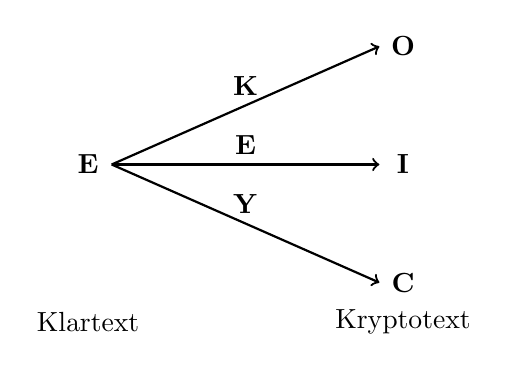
\begin{tikzpicture}
	    % Klartext und Kryptotext Labels
	    \node at (0, 0) {\textbf{E}};
	    \node at (4, 1.5) {\textbf{O}};
	    \node at (4, 0) {\textbf{I}};
	    \node at (4, -1.5) {\textbf{C}};
	
	    % Verbindungspfeile mit Schlüsseln
	    \draw[->, thick] (0.3, 0) -- (3.7, 1.5) node[midway, above] {\textbf{K}};
	    \draw[->, thick] (0.3, 0) -- (3.7, 0) node[midway, above] {\textbf{E}};
	    \draw[->, thick] (0.3, 0) -- (3.7, -1.5) node[midway, above] {\textbf{Y}};
	
	    % Labels Klartext und Kryptotext
	    \node[align=center] at (0, -2) {Klartext};
	    \node[align=center] at (4, -2) {Kryptotext};
	\end{tikzpicture}}
	\end{subfigure}
	\begin{subfigure}{.35\textwidth}
	\centering
	\resizebox{\textwidth}{!}{
	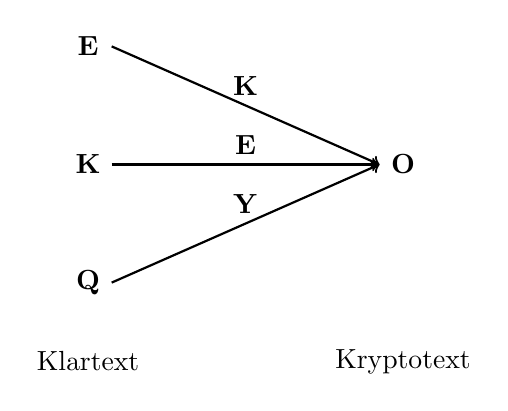
\begin{tikzpicture}
	    % Klartext letters
	    \node at (0, 1.5) {\textbf{E}};
	    \node at (0, 0) {\textbf{K}};
	    \node at (0, -1.5) {\textbf{Q}};
	    
	    % Kryptotext letter
	    \node at (4, 0) {\textbf{O}};
	    
	    % Verbindungspfeile mit Schlüsseln
	    \draw[->, thick] (0.3, 1.5) -- (3.7, 0) node[midway, above] {\textbf{K}};
	    \draw[->, thick] (0.3, 0) -- (3.7, 0) node[midway, above] {\textbf{E}};
	    \draw[->, thick] (0.3, -1.5) -- (3.7, 0) node[midway, above] {\textbf{Y}};
	    
	    % Labels Klartext und Kryptotext
	    \node[align=center] at (0, -2.5) {Klartext};
	    \node[align=center] at (4, -2.5) {Kryptotext};
	\end{tikzpicture}}
	\end{subfigure}
	\end{figure}
	}

\begin{frame}[label=title]
    \centering
    \begin{figure}[H]
        
\includegraphics[keepaspectratio, width=0.7\paperwidth, height=\paperheight]{Logos/LeeLogo}
    \end{figure}
    Informatik: Data Science und Sicherheit\\
    \emoji{chart-increasing}: \textbf{Kryptoanalyse}
\end{frame}


\begin{frame}[label=repetition]{Geheimschriften: \emoji{cat}- und \emoji{mouse}-Rennen}
	\begin{multicols}{2}
		\textbf{Kryptologie}
		\begin{itemize}
			\item Geheimschrift mit vertauschten Buchstaben
			\item Skytale
			\item Caesar
		\end{itemize}
		\columnbreak
		\textbf{Kryptoanalyse}
		\begin{itemize}
			\item Geheimschriften analysieren
			\item 26 Verschiebungen ausprobieren
			\item Statistische Analyse
		\end{itemize}
	\end{multicols}
\end{frame}

\begin{frame}[label=repetition2]{Wiederholung letztes Mal}
	\begin{figure}[H]
		\centering
		\raisebox{-0.5\height}{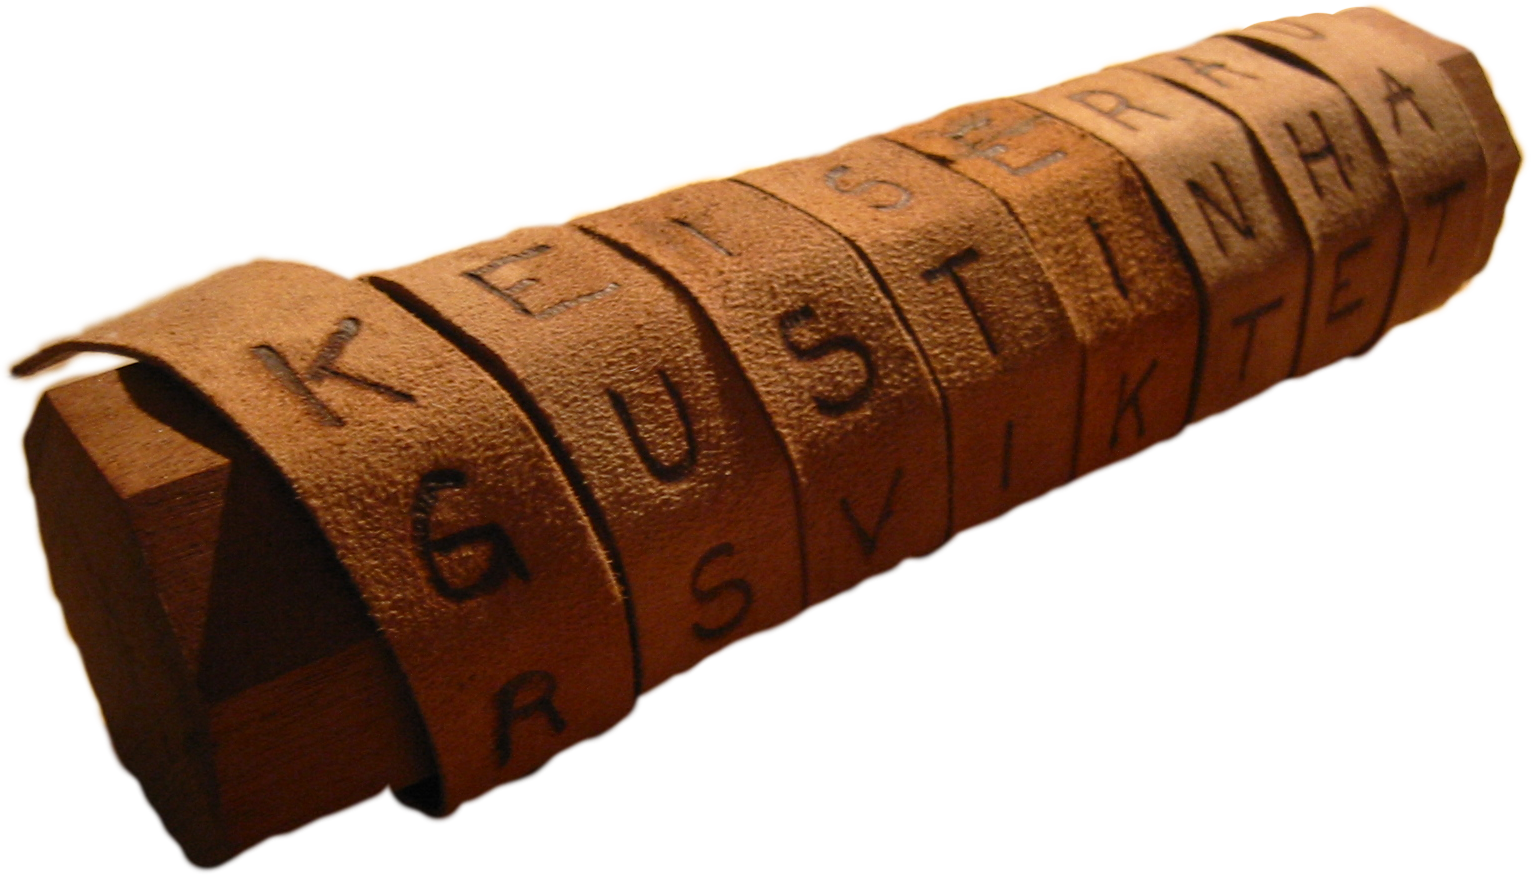
\includegraphics[width=.35\linewidth]{GrundlagenInfo/03_Kryptologie/Figures/SkytaleWiki}}
		\raisebox{-0.5\height}{$\rightarrow$ Tabellengrössen ausprobieren}
		\raisebox{-0.5\height}{\resizebox{.35\linewidth}{!}{\caesar[6]}}
		\raisebox{-0.5\height}{$\rightarrow$ 26 Verschiebungen ausprobieren}
	\end{figure}

\end{frame}

\begin{frame}[label=caesarex, fragile]{Wiederholung letztes Mal: Angriff auf Caesar}
	\centering
	Wie würden Sie folgenden Text knacken?\\[.5cm]
	    \defverbatim{\verbOne}{
\small\begin{verbatim}
Geheimtext: PKSGTJSAYYZKPUYKLQBKXRKASJKZNG...
\end{verbatim}
	        }
 \defverbatim{\verbTwo}{
	      \small\begin{verbatim}
  Klartext: JEMANDMUSSTEJOSEFKVERLEUMDETHA...
 Schlüssel: GGGGGGGGGGGGGGGGGGGGGGGGGGGGGG...
Geheimtext: PKSGTJSAYYZKPUYKLQBKXRKASJKZNG...
	      \end{verbatim}
	      }
	    \only<1-5>{\verbOne}
	    \only<2-4>{
	    Häufigster Buchstabe im obigen Geheimtext: \texttt{K}\\
	    Häufigster Buchstabe im deutschen Alphabet: \texttt{E}
	    }
	    
	 \only<3-5>{
	 \begin{itemize}
	   \item<3-5> \texttt{E} = Buchstabe 4
	   \item<4-5> \texttt{K} = Buchstabe 10
	   \item<5> Schlüssel $=$ Verschiebung von $10-4 = 6 =$ Buchstabe \texttt{G}
	 \end{itemize}	 
	 }
	 \only<5-6>{
	 \centering\scalebox{.5}{\caesar[6]}
	 }
	 
	 \only<6>{\verbTwo}	
\end{frame}

\begin{frame}[fragile]{Häufigkeitsverteilung}
		\begin{figure}[H]
			\centering
			\multiKey{Z,E,A,B,C,D,Y,X,W,H,I,V,U,T,G,F,J,K,R,Q,L,M,S,N,P,O}
			$\rightarrow$ \textbf{Wie knacken wir so etwas?}
		\end{figure}
\end{frame}

\begin{frame}[fragile, label=hauefigkeit]{Häufigkeitsverteilung}
	\begin{multicols}{2}
		    \begin{figure}[H]
			\centering
			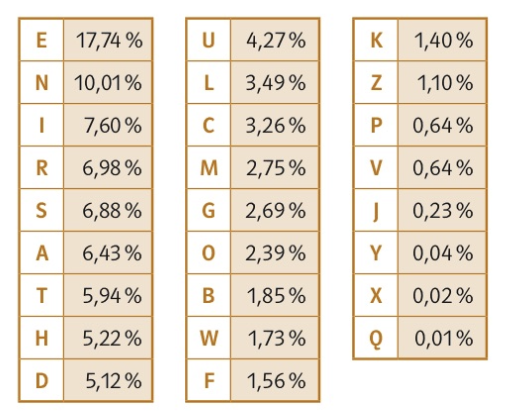
\includegraphics[width=\linewidth]{GrundlagenInfo/03_Kryptologie/Figures/freq.png}
		\end{figure}
		\columnbreak
		\[h_\square (T)\]
		= Häufigkeit von Buchstabe $\square$ in Text $T$.
	\end{multicols}
    \begin{figure}[H]
    	\centering
    	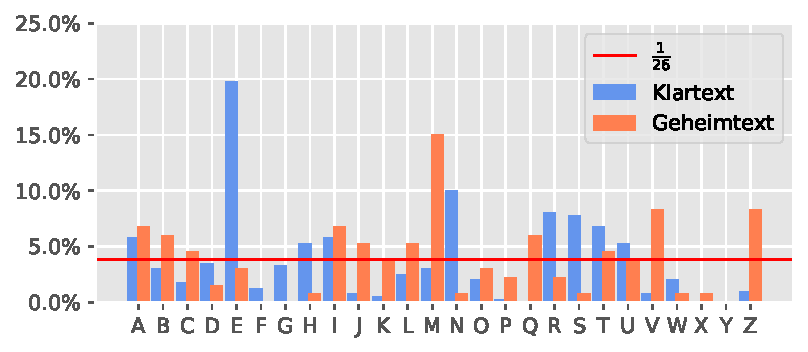
\includegraphics[width=.7\textwidth]{GrundlagenInfo/03_Kryptologie/Figures/letterfreq_end_dec0}
    \end{figure}
\end{frame}


\begin{frame}[fragile]{Häufigkeitsanalyse}
\textbf{Problem}: Alle \textbf{monoalphabetischen} Kryptosysteme lassen sich mit einfacher Häufigkeitsanalyse knacken
    \begin{figure}[H]
        \centering
        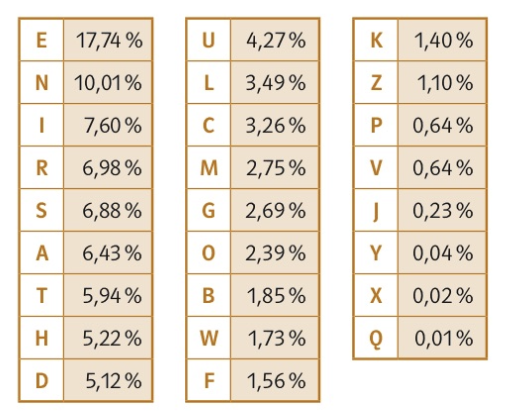
\includegraphics[width=.5\linewidth]{GrundlagenInfo/03_Kryptologie/Figures/freq.png}
        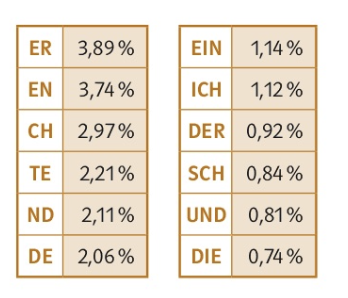
\includegraphics[width=.35\linewidth]{GrundlagenInfo/03_Kryptologie/Figures/bigramme.png}
    \end{figure}
    %\textcolor{red}{\rule{\textwidth}{.3mm}}\\[-.1cm]
    \defverbatim{\verbOne}{
    \small\begin{verbatim}
MUMMUXJUQYMHQOUSUTUQNGWTJQVHUMXQUXQJSUVYPPUM
--------------------------------------------
    \end{verbatim}
    U kommt 10-mal vor, M kommt 6-mal vor, Q kommt 6-mal vor}
    \defverbatim{\verbTwo}{
    \small\begin{verbatim}
MUMMUXJUQYMHQOUSUTUQNGWTJQVHUMXQUXQJSUVYPPUM
NENNE--EI-N-I-E-E-EI-----I--EN-IE-I--E----EN
    \end{verbatim}
    U=E, M=N, Q=I?
    }
    \defverbatim{\verbThree}{
    \small\begin{verbatim}
MUMMUXJUQYMHQOUSUTUQNGWTJQVHUMXQUXQJSUVYPPUM
NENNED-EI-N-I-E-E-EI-----I--ENDIEDI--E----EN
\end{verbatim}
Wir fahren nun mit Trigrammen weiter: ``Die''?}
    \defverbatim{\verbFour}{
    \small\begin{verbatim}
MUMMUXJUQYMHQOUSUTUQNGWTJQVHUMXQUXQJSUVYPPUM
NENNEDREI-N-I-E-E-EI----RI--ENDIEDIR-E----EN
\end{verbatim}
``D-EI''=``Drei''?}
    \defverbatim{\verbFive}{
    \small\begin{verbatim}
MUMMU|XJUQ|YMHQOUSUTUQNGWTJQVHUM|XQU|XQJ|SUVYPPUM
NENNE|DREI|-N-I-E-E-EI----RI--EN|DIE|DIR|-E----EN
\end{verbatim}
	Man beginnt einzelne Wörter zu erkennen...
    }
    \defverbatim{\verbSix}{
    \small\begin{verbatim}
MUMMU|XJUQ|YMHQOU|SUTUQNGWTJQVHUM|XQU|XQJ|SUVYPPUM
NENNE|DREI|ANTIKE|GEHEIMSCHRIFTEN|DIE|DIR|GEFALLEN
    \end{verbatim}
    \emoji{blush}
    }
    \only<1>{\verbOne}
    \only<2>{\verbTwo}
    \only<3>{\verbThree}
    \only<4>{\verbFour}
    \only<5>{\verbFive}
    \only<6>{\verbSix}
\end{frame}

\begin{frame}[label=auftrag]{Auftrag}
Skript
\begin{itemize}
   \item \aufgabebox{1.9}
   \item \challengebox{1.10, 1.11}
\end{itemize}
\end{frame}

\begin{frame}{Mono- und Polyalphabetische Kryptosysteme}
	\begin{itemize}[<+->]
		\item \textbf{Monoalphabetisch}: Jeder Buchstabe wird immer durch denselben Buchstaben erstetzt, unabhängig von seiner Position im Klartext. \textbf{Nachteil}: Einfache Entschlüsselung durch Häufigkeitsanalyse
		\item \textbf{Polyalphabetisch}: Jeder Buchstabe kann durch unterschiedliche Buchstaben ersetzt werden
	\end{itemize}
\end{frame}

%\begin{frame}{Kerkhoffs'sches Prinzip der Sicherheit}
%	\begin{center}
%		``Ein Kryptosystem ist \textbf{sicher}, wenn das Kryptosystem [= der Algorithmus] öffentlich bekannt ist und es trotzdem ohne die Kenntnis des verwendeten Schlüssels nicht möglich ist, aus einem Geheimtext den ursprünglichen Klartext abzuleiten.''
%	\end{center}    
%\end{frame}

\begin{frame}[label=vigenere, fragile]{Vigenère \emoji{fleur-de-lis}}
\defverbatim{\verbOne}{
Von Caesar...
\begin{verbatim}
  Klartext: JEMANDMUSSTEJOSEFKVERLEUMDETHA...
 Schlüssel: GGGGGGGGGGGGGGGGGGGGGGGGGGGGGG...
Geheimtext: PKSGTJSAYYZKPUYKLQBKXRKASJKZNG...
\end{verbatim}
}
    
\only<1>{\verbOne}
\defverbatim{\verbTwo}{
\begin{verbatim}
  Klartext: JEM|AND|MUS|STE|JOS|EFK|VER|LE...
 Schlüssel: KEY|KEY|KEY|KEY|KEY|KEY|KEY|KE...
Geheimtext: TIK|KRB|WYQ|CXC|TSQ|OJI|FIP|VI...
\end{verbatim}
    }

    \only<2>{...zu Vigenère}
    \only<2->{\verbTwo}
	
\only<3>{
	\begin{itemize}
	    \item B=Verschiebung um 1 Position, C=Verschiebung um 2 Positionen, usw.
	    \item Allgemein: Verschiebung = $\text{Ord}(\square)$, wobei $\text{Ord}(A)=0$
	    \item nicht \textbf{monoalphabetisch} sondern \textbf{polyalphabetisch}
	    \item Galt über 300 Jahre lang als sicher!
	\end{itemize}
	\vigenereFig
	}
\end{frame}

\begin{frame}{Vigenère-Tabelle}
\begin{figure}[H]
\centering
\resizebox{.75\linewidth}{!}{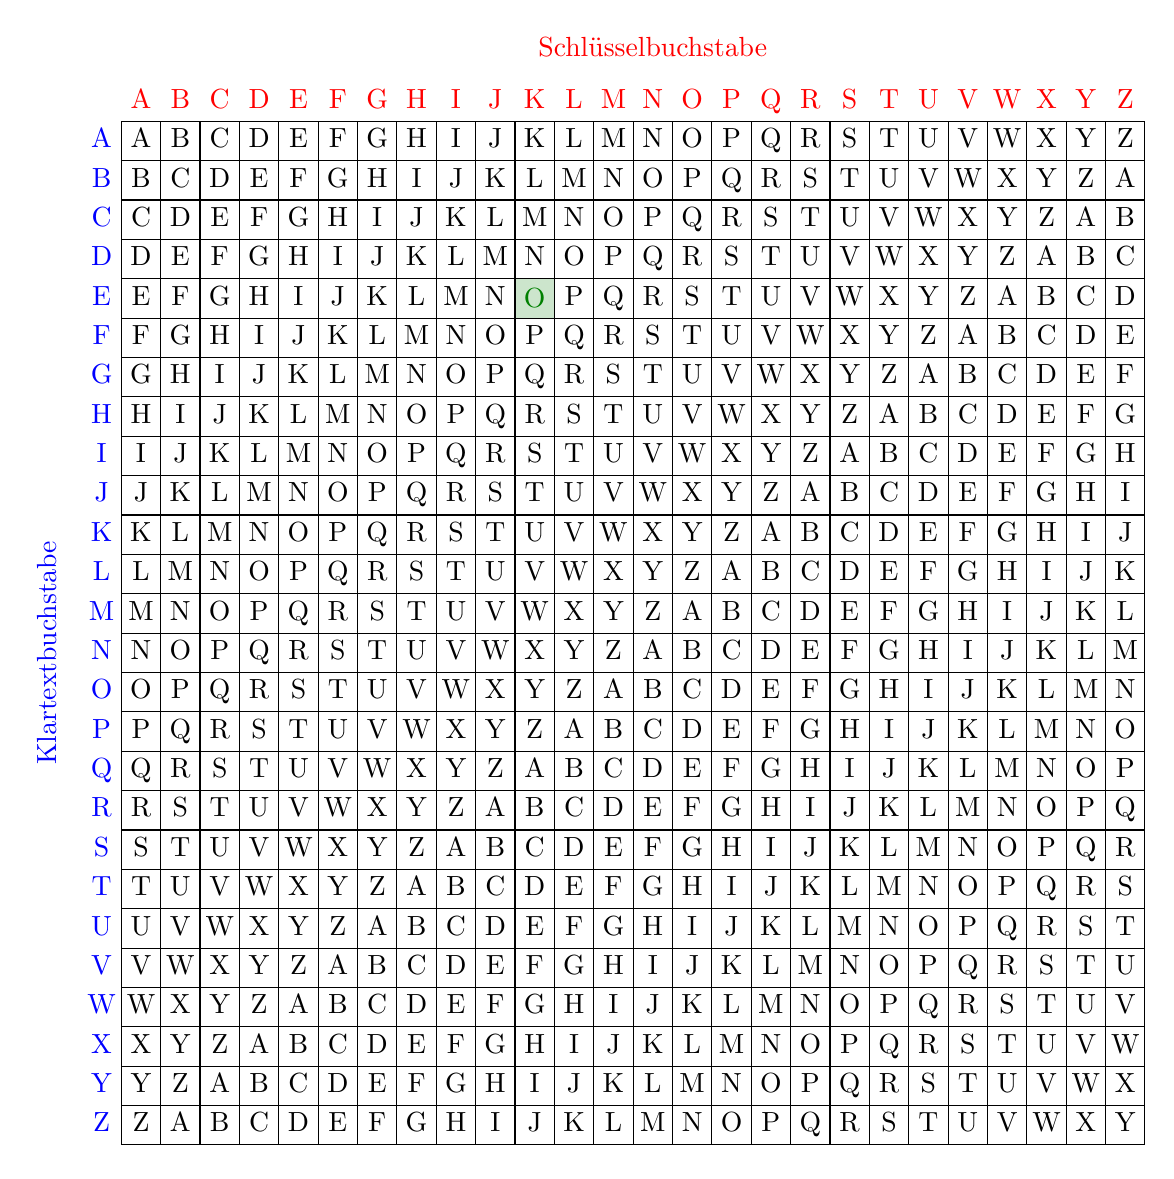
\begin{tikzpicture}
\foreach \i in {0,...,25} {
    \node at (-0.5,-\i*0.5) {\textcolor{Blue}{\strut\symbol{\numexpr`A+\i\relax}}};
    \node at (\i*0.5,0.5) {\textcolor{Red}{\strut\symbol{\numexpr`A+\i\relax}}};
  \foreach \j in {0,...,25} {
    \edef\k{\ifnum\numexpr\i+\j\relax>25
        \the\numexpr\i+\j-26\relax
      \else
        \the\numexpr\i+\j\relax
      \fi}
  \node[draw,minimum size=0.5cm,inner sep=0pt]
    at (\i*0.5,-\j*0.5) {\strut\symbol{\numexpr`A+\k\relax}};
  }
}
\node[draw,minimum size=0.5cm,inner sep=0pt,fill=Green!20] at (5.0,-2.0) {\textcolor{Green}{O}};
\node at (6.5,1.2) {\textcolor{Red}{Schlüsselbuchstabe}};
\node[rotate = 90] at (-1.2,-6.5)  {\textcolor{Blue}{Klartextbuchstabe}};
\end{tikzpicture}}
\end{figure}
\end{frame}


\begin{frame}[label=vigenere2]{Vigenère \emoji{fleur-de-lis}}
	\vigenereFig
	\begin{align*}
	    h_{Geheimtext}(O) &= \frac{h_{Klartext}(E)+h_{Klartext}(K)+h_{Klartext}(Q)}{3} \\
	    &= \frac{17.7\%+1.4\%+0.01\%}{3}=6.4\%
	\end{align*}
	$\rightarrow$ Die Häufigkeiten der Buchstaben entsprechen nun nicht mehr direkt einer Häufigkeit eines anderen Buchstabens im Originaltext!
\end{frame}
\begin{frame}[label=keyFixed]{Angriff auf Vigenère: Bekannte Schlüssellänge}
	\texttt{\colorstring[ForestGreen,RoyalBlue,Crimson]{RGTIPKUWZAVLRQZMHRDGYTGBUFLBJHJGULGUVQOVGKIUZMTLBYHADAAGZOGAIPOJVAMYBZFLMTLQPLAOVZILVUCMTOIHAMVZEKLMKUPWULWJACNBGLZGZEC...}}
			
\foreach \cae/\fignum/\i/\colorgroup/\lettergroup in {8/0/1/ForestGreen/M,2/1/2/RoyalBlue/G,7/2/3/Crimson/L} {
	\only<\i>{
	$\rightarrow$ Häufigster Buchstaben in Gruppe \i: \textcolor{\colorgroup}{\lettergroup}
	\begin{figure}[H]
		\centering
		\raisebox{-0.5\height}{\includegraphics[width=.75\linewidth]{GrundlagenInfo/03_Kryptologie/Figures/letterfreq_end_dec\fignum}}
		\raisebox{-0.5\height}{\resizebox{.23\textwidth}{!}{\caesar[\cae]}}
	\end{figure}
	}
}
\end{frame}



\begin{frame}[label=keyFixed]{Angriff auf Vigenère: Bekannte Schlüssellänge}
	\textbf{Beispiel}: Geheimtext mit Schlüssellänge 3
	\only<1>{
	\begin{figure}[H]
	        \centering
	        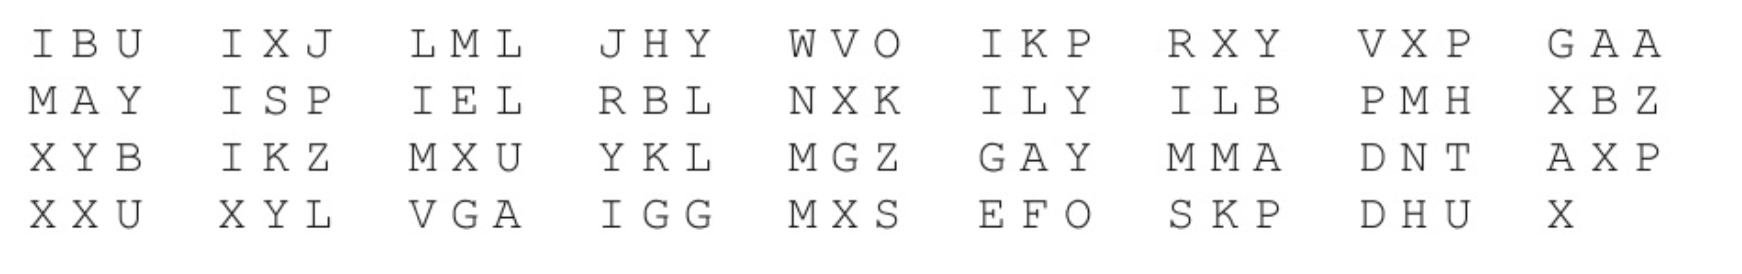
\includegraphics[width=\linewidth]{GrundlagenInfo/03_Kryptologie/Figures/vigenereKeyFixed1.png}
	\end{figure}
	}
	
	\only<2->{
	\begin{figure}[H]
	        \centering
	        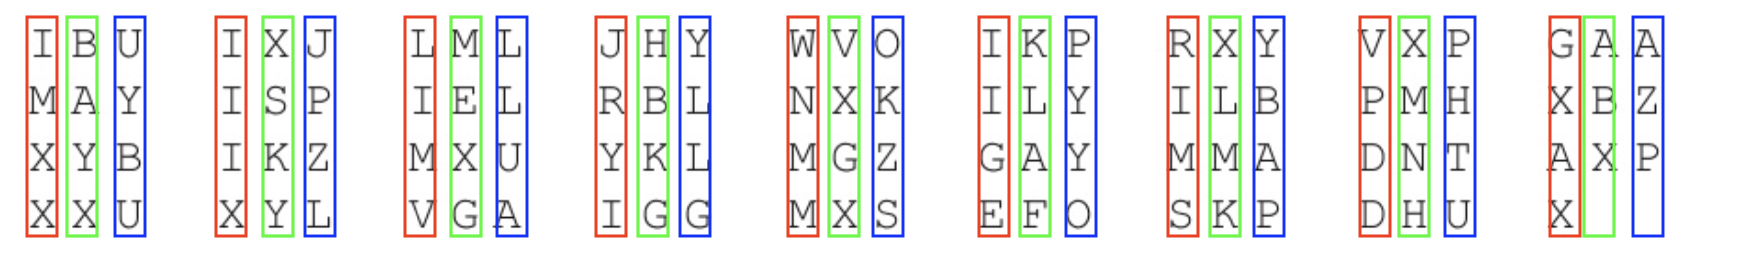
\includegraphics[width=\linewidth]{GrundlagenInfo/03_Kryptologie/Figures/vigenereKeyFixed2.png}
	\end{figure}
	}
	\only<3>{\textbf{Häufigkeitsanalyse} pro Gruppe (rot, grün, blau):\\
	\begin{figure}[H]
	        \centering
	        \raisebox{-0.5\height}{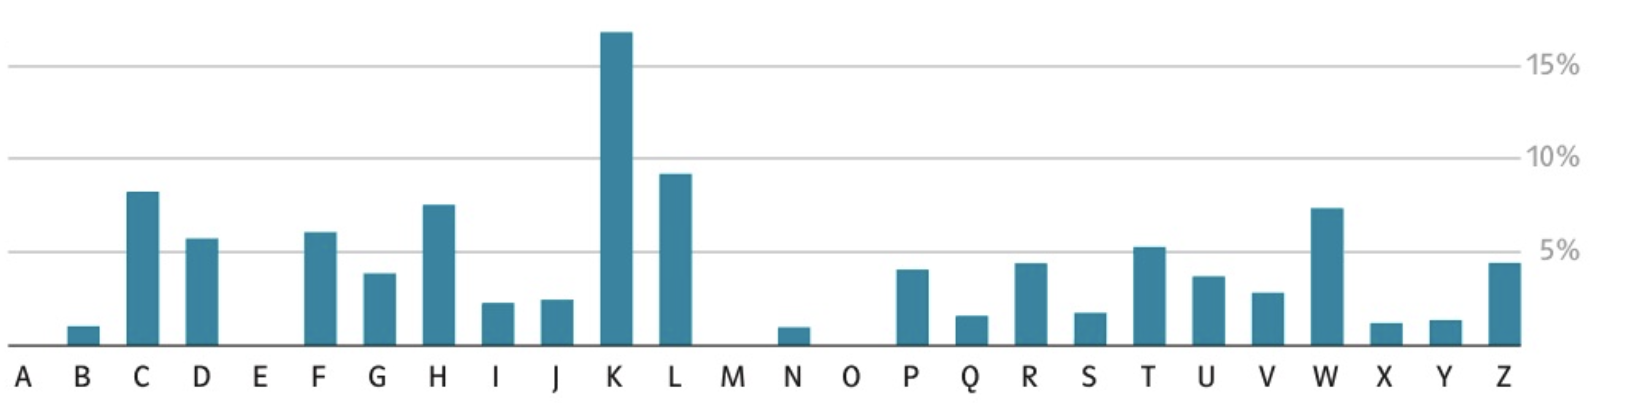
\includegraphics[width=.45\textwidth]{GrundlagenInfo/03_Kryptologie/Figures/friedmann1-geheimtext.png}}
	        \raisebox{-0.5\height}{$\rightarrow$}
	        \raisebox{-0.5\height}{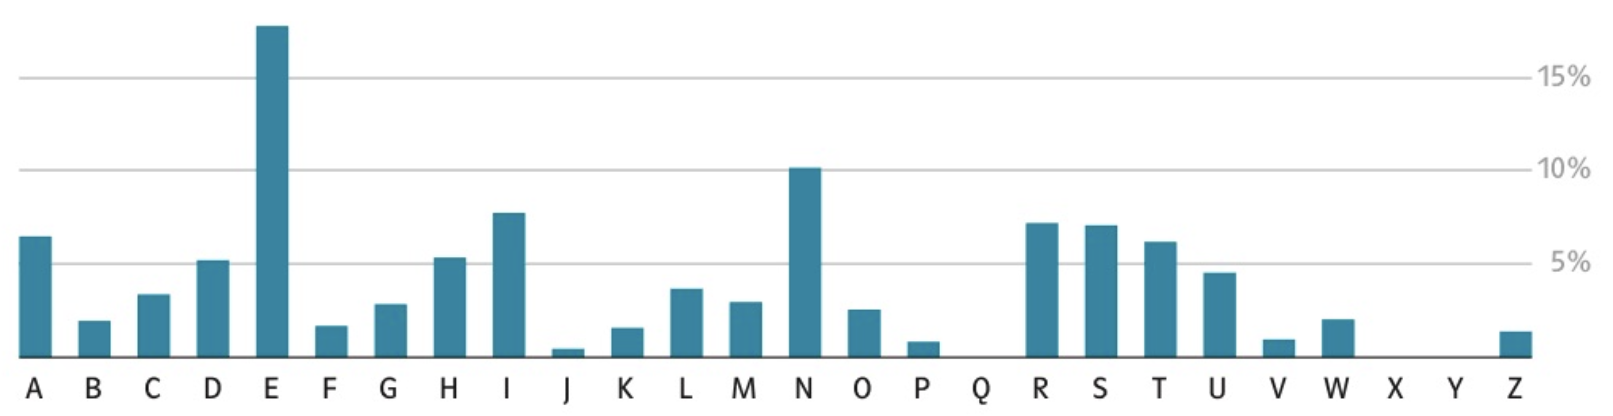
\includegraphics[width=.45\textwidth]{GrundlagenInfo/03_Kryptologie/Figures/friedmann1-klartext.png}}
	\end{figure}}
\end{frame}

\begin{frame}[label=auftrag]{Auftrag}
	\begin{itemize}
		\item \aufgabebox{1.12}
		\item \aufgabebox{1.13}
		\item \aufgabebox{1.14}
	\end{itemize}
\end{frame}

\begin{frame}[fragile,label=friedmann]{Friedmann'sche Charakteristik}
Wie kann man die Schlüssellänge herausfinden, falls diese unbekannt ist?$\rightarrow$ \textbf{Idee:}
	\begin{itemize}\only<1>{
	
	\item<1> Die Häufigkeit der Buchstaben in einem Vigenère-Geheimtext ist wegen der \textit{polyalphabetischen} Verschlüsselung relativ \textit{gleichmässig}...
		\begin{figure}[H]
				\centering
				\raisebox{-0.5\height}{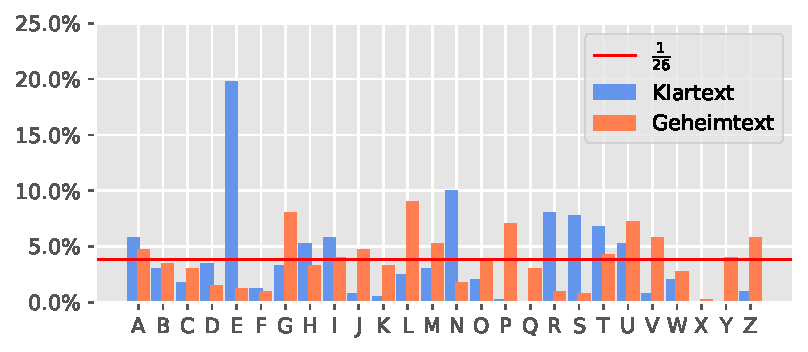
\includegraphics[width=.75\linewidth]{GrundlagenInfo/03_Kryptologie/Figures/letterfreq_end_dec_alletters}}
			\end{figure}}
			\only<2->{
	\item<2-> ...ausser wir schauen die Buchstaben eben in \colorstring[ForestGreen,RoyalBlue,Crimson]{Gruppen} an!
		\begin{figure}[H]
			\centering
			\raisebox{-0.5\height}{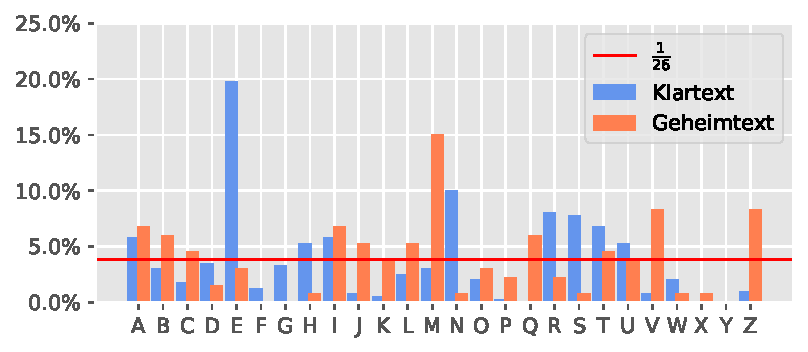
\includegraphics[width=.45\linewidth]{GrundlagenInfo/03_Kryptologie/Figures/letterfreq_end_dec0}}
			\raisebox{-0.5\height}{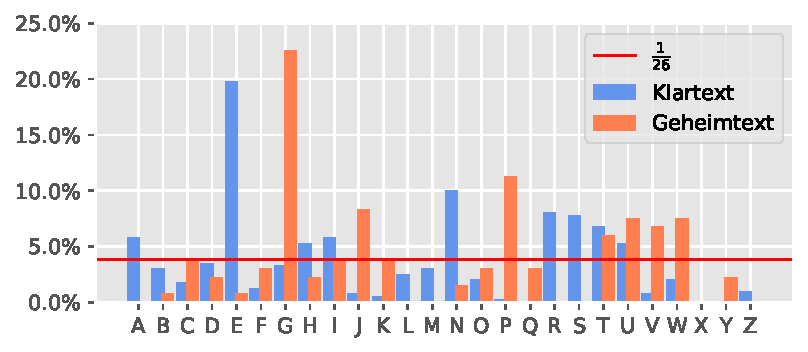
\includegraphics[width=.45\linewidth]{GrundlagenInfo/03_Kryptologie/Figures/letterfreq_end_dec1}}
			\raisebox{-0.5\height}{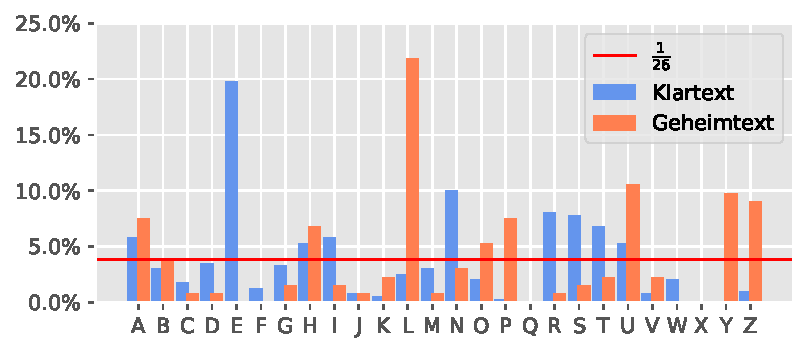
\includegraphics[width=.45\linewidth]{GrundlagenInfo/03_Kryptologie/Figures/letterfreq_end_dec2}}\\
			(Schrittgrösse=3)
		\end{figure}
		
	\item<3> Kann man für die ``(Un-)Gleichmässigkeit'' der Verteilung eine einzige ``Zahl'' erfinden?}
		\end{itemize}
\end{frame}

\begin{frame}[fragile,label=friedmann]{Friedmann'sche Charakteristik}
	\begin{figure}[H]
	        \centering
	        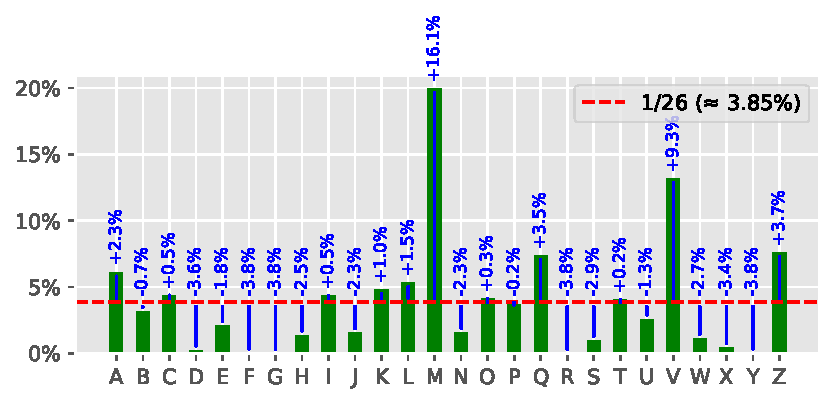
\includegraphics[width=\textwidth]{GrundlagenInfo/03_Kryptologie/Figures/vigenere-len3-group1-avg}
	\end{figure}
	\only<2>{
	\begin{align*}
	    FC(T)&=\Big(h_A(T)-\frac{1}{26}\Big)^2+\Big(h_B(T)-\frac{1}{26}\Big)^2+\ldots+\Big(h_Z(T)-\frac{1}{26}\Big)^2\\
	    &=\sum_{\Delta\in \text{Alphabet}}\Big(h_\Delta(T)-\frac{1}{26}\Big)^2
	\end{align*}
	\emoji{flag-germany} $FC(T)\sim 0.0388$ für deutsche Texte 
	}
\end{frame}

\begin{frame}{Angriff auf Vigenère: Beispiel}{Friedmann'sche Charakteristik + Häufigkeitsanalyse}
\texttt{MUZKJLQPAWJUMHYIILLCZAUPMRLZHLSVCMTZBCULGUPCIMPDQGTIP\\
		CQILVGYMGUBUJPNBMUZMNAPGYHNPKJLOTHBWSIVPWPKIHB...}\\[.2cm]
	\only<2-9>{
		\textit{Brute force}-Ansatz, um Wortlänge von Vigenère zu berechnen: 
	\begin{enumerate}[<+->]
		    \item Alle möglichen Schlüsselwortlängen von 1 bis $n$ ausprobieren
		    \item Buchstaben jeweils in Gruppen unterteilen
		    \begin{itemize}
		   		\scriptsize
		   		\item 2 Gruppen: \texttt{\colorstring[ForestGreen,RoyalBlue]{MUZ KJL QPA WJU MHY IIL LCZ AUP MRL ZHL SVC 
		   						MTZ BCU LGU PCI MPD QGT IPC QIL VGY MGU BUJ 
		   						PNB MUZ MNA PGY HNP KJL OTH BWS IVP WPK IHB}}
		   		\item 3 Gruppen: \texttt{\colorstring[ForestGreen,RoyalBlue,Crimson]{MUZ KJL QPA WJU MHY IIL LCZ AUP MRL ZHL SVC 
		   		MTZ BCU LGU PCI MPD QGT IPC QIL VGY MGU BUJ
		   		PNB MUZ MNA PGY HNP KJL OTH BWS IVP WPK IHB}}
		   		\item 4 Gruppen: \texttt{\colorstring[ForestGreen,RoyalBlue,Crimson,LightSlateBlue]{MUZ KJL QPA WJU MHY IILLCZ AUP MRL ZHL SVC MTZ BCU LGU PCI MPD QGT IPC QIL VGY MGU BUJ PNB MUZ MNA PGY HNP KJL OTH BWS IVP WPK IHB}}
		   		\item ...
		   	\end{itemize}
		    \item Durchschnittliche $FC(T)$ für alle Gruppen pro Schlüssellänge berechnen. 
		    \item Wenn die richtige Schlüssellänge gewählt wurde, sollte $FC(T)\sim 0.0388$ sein.
		\end{enumerate}}
	    
\only<10>{	
		\begin{figure}[H]
			\centering
			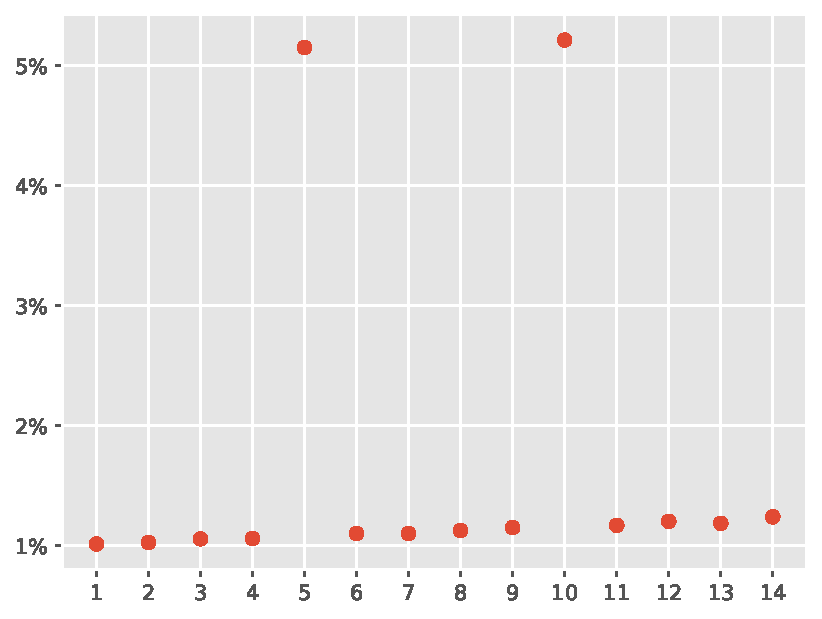
\includegraphics[width=.65\textwidth]{GrundlagenInfo/03_Kryptologie/Figures/friedman}
		\end{figure}
	$\rightarrow$ Zeigt, wie ungleich die Buchstaben verteilt sind, wenn wir sie in 1, 2, 3, 4, ... Gruppen aufteilen.\\
	$\rightarrow$ Hier sehen wir visuell, dass die Wortlänge 3 sein muss.}
\end{frame}

\begin{frame}{Angriff auf Vigenère: Beispiel}{Friedmann'sche Charakteristik + Häufigkeitsanalyse}
\texttt{\colorstring[ForestGreen,RoyalBlue,Crimson]{MUZ KJL QPA WJU MHY IIL LCZ AUP MRL ZHL SVC 
		MTZ BCU LGU PCI MPD QGT IPC QIL VGY MGU BUJ 
		PNB MUZ MNA PGY HNP KJL OTH BWS IVP WPK IHB}}
		
		$\rightarrow$ Häufigster Buchstaben pro Gruppe: \textcolor{ForestGreen}{M}, \textcolor{RoyalBlue}{G}, \textcolor{Crimson}{L}
		
		\begin{figure}[H]
			\centering
			\resizebox{.75\textwidth}{!}{\caesar[8] \caesar[2] \caesar[7]}
		\end{figure}
\end{frame}

\begin{frame}[label=auftrag]{Auftrag}
	\begin{itemize}
		\item \aufgabebox{1.15}
		\item \aufgabebox{1.16}
		\item \aufgabebox{1.17}
		\item \aufgabebox{1.18}
		\item \challengebox{1.19,1.20}
	\end{itemize}
\end{frame}

\begin{frame}[fragile]{Appendix}
Anhang
\end{frame}


\begin{frame}[fragile]{Vigenère in Python}
\begin{lstlisting}[language=Python,basicstyle=\ttfamily\tiny]
def caesar_buchstabe(buchstabe, verschiebung):
    return chr((ord(buchstabe) - ord("A") + verschiebung) % 26 + ord("A"))


def caesar(text, verschiebung):
    text_verschoben = ""

    for buchstabe in text:
        text_verschoben += caesar_buchstabe(buchstabe, verschiebung)

    return text_verschoben

def vigenere(text, schluessel, richtung="verschluesslung"):
    text_verschoben = ""
    k = 0
    for buchstabe in text:
        k %= len(schluessel)
        if richtung == "verschluesslung":
            text_verschoben += caesar_buchstabe(
                buchstabe, ord(schluessel[k]) - ord("A")
            )
        else:
            text_verschoben += caesar_buchstabe(
                buchstabe, -(ord(schluessel[k]) - ord("A"))
            )
        k += 1

    return text_verschoben
\end{lstlisting}
\end{frame}


\begin{frame}[label=kasiski]{Angriff auf Vigenère: Unbekannte Schlüssellänge}{\textbf{Kasiski-Test}}
\emoji{key} Schlüssellänge unbekannt!\\[1cm]
\texttt{DER KLAR\textbf{TEXT} WERDE GEHEIM\textbf{TEXT}\\
PLU TOPL\textbf{UTOP} LUTOP LUTOPL\textbf{UTOP}\\
SPL DZPC\textbf{NXLI} HYKRT RYASXX\textbf{NXLI}}\\[1cm]

\begin{itemize}
    \item ``\texttt{NXLI}'' kommt zweimal im Geheimtext vor
    \item Distanz zwischen \texttt{NXLI} = Vielfaches der Schlüssellänge
\end{itemize}
\end{frame}
\begin{frame}[label=kasiski2]{Angriff auf Vigenère: \textbf{Kasiski-Test}}
\only<1>{
Angenommen, wir haben folgenden Text, verschlüsselt mit dem Wort ``BALMER'':
\begin{figure}[H]
        \centering
        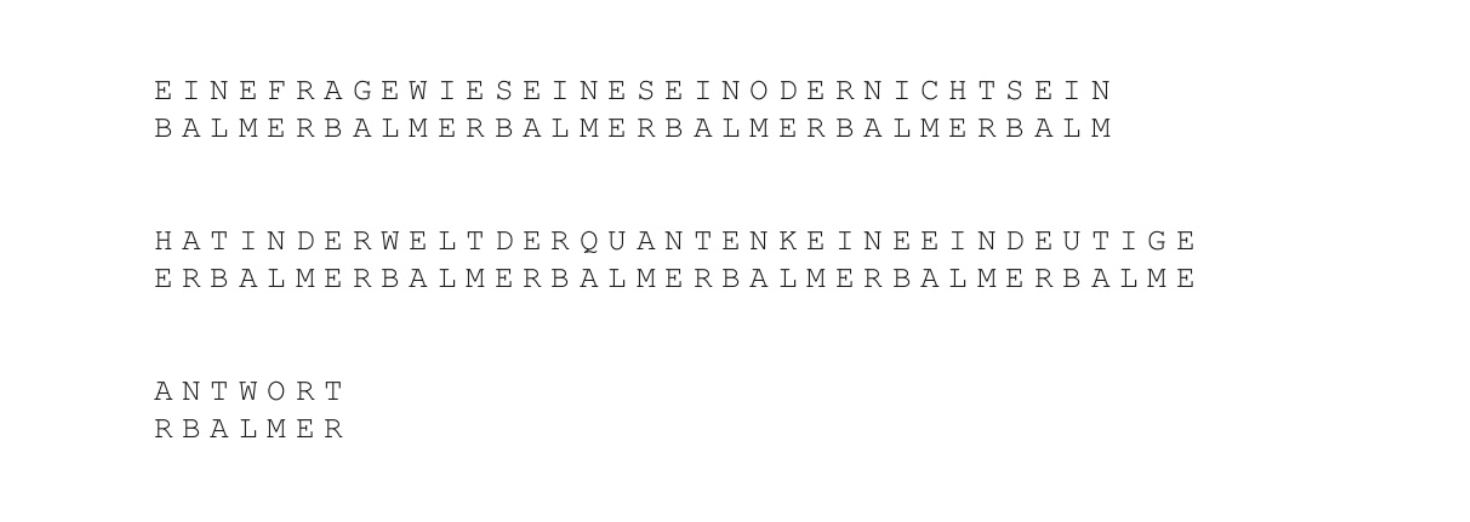
\includegraphics[width=\textwidth]{GrundlagenInfo/03_Kryptologie/Figures/Kasiski1.png}
\end{figure}
}
\only<2>{
Wir suchen nun zuerst im Geheimtext nach Trigrammen, die mehrmals vorkommen:
\begin{figure}[H]
        \centering
        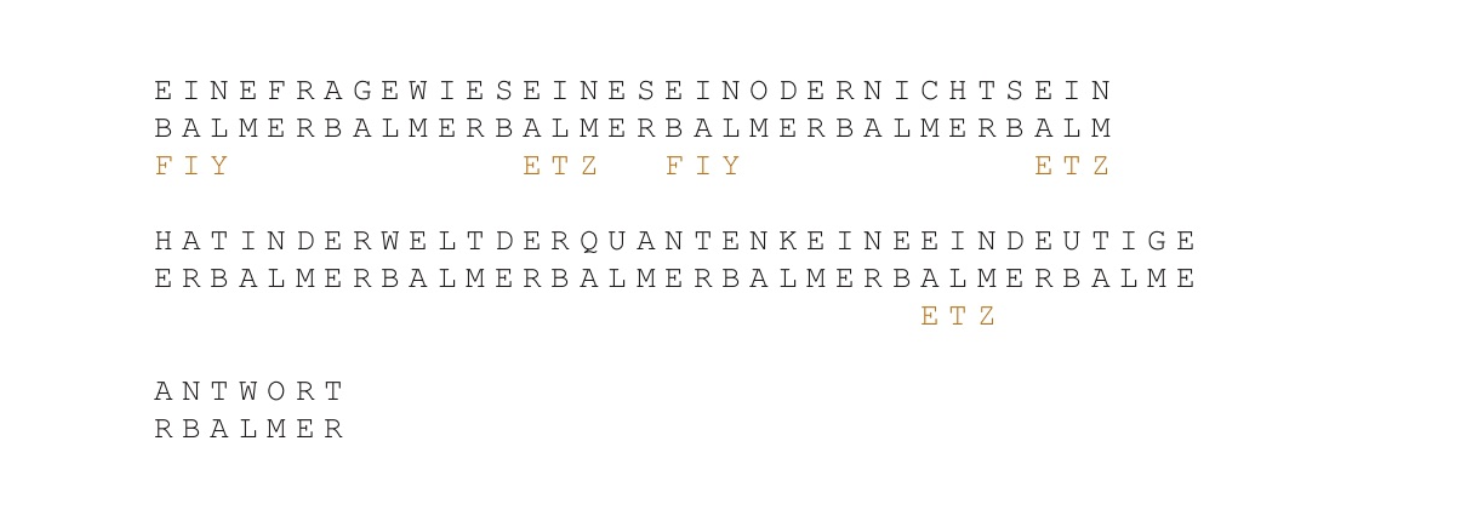
\includegraphics[width=\textwidth]{GrundlagenInfo/03_Kryptologie/Figures/Kasiski2.png}
\end{figure}
}
\only<3>{
Wir notieren die Anfangs-Positionen der Trigramme:
\begin{figure}[H]
        \centering
        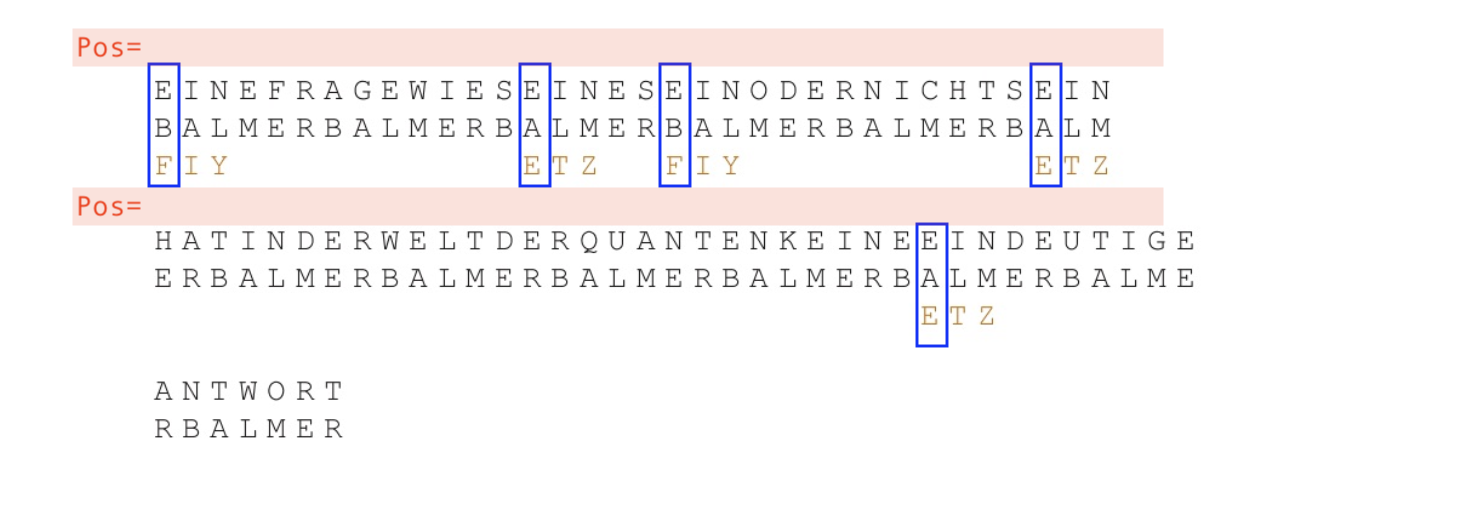
\includegraphics[width=\textwidth]{GrundlagenInfo/03_Kryptologie/Figures/Kasiski3.png}
\end{figure}
}
\only<4->{
Wir notieren die Anfangs-Positionen der Trigramme:
\begin{figure}[H]
        \centering
        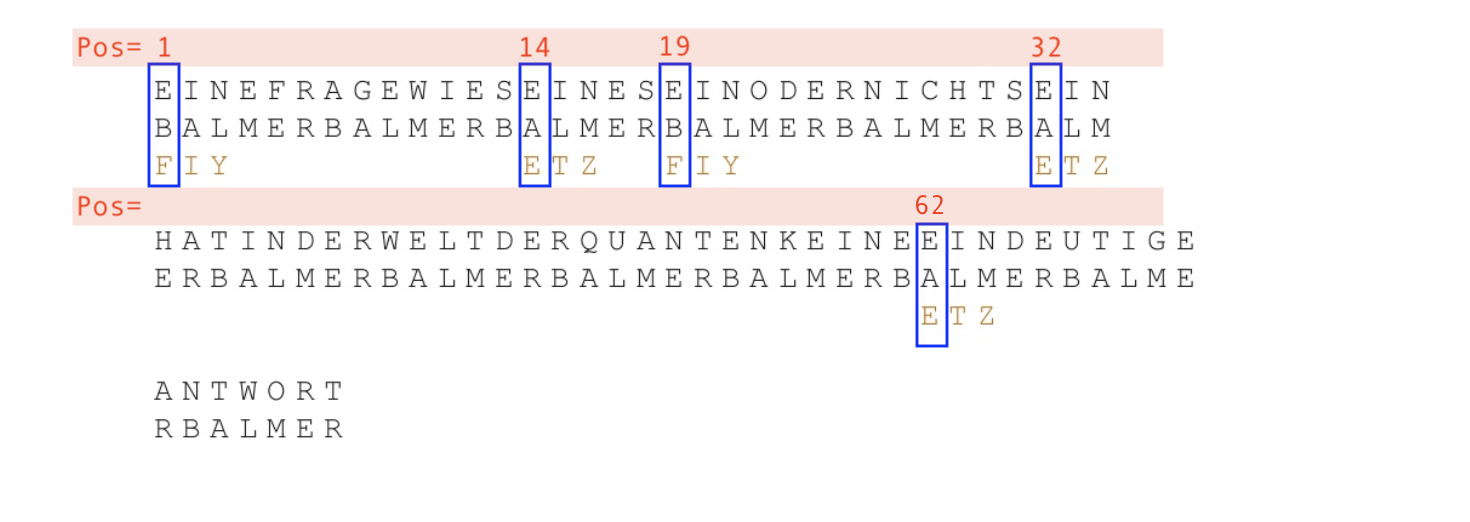
\includegraphics[width=\textwidth]{GrundlagenInfo/03_Kryptologie/Figures/Kasiski4.png}
\end{figure}
}
\only<5->{
Nun können wir die Abstände zwischen den mehrfach vorkommenden Trigrammen berechnen:
\begin{align*}
62 - 14 = 48 = 2^4\cdot 3\\
62 - 32 = 30 = 2 \cdot 3 \cdot 5\\
32 - 14 = 18 = 2 \cdot 3^2
\end{align*}
GGT = 6 $\rightarrow$ Länge des Schlüsselworts.
}
\end{frame}